% !TeX root = ../libro.tex
% !TeX encoding = utf8



\setchapterpreamble[c][0.90\linewidth]{%
	\sffamily
  
    Entre 1950 y 1960 fueron los años en los cuales destaca la publicación de un artículo de Alan Turing, \textit{Maquinaria computacional e Inteligete}, y el nacimiento del perceptrón a manos de Frank Rosenblatt inspirado por el trabajo de otros autores como Warren MCCulloch y Walter Pitss, precursando el campo de la inteligencia artificial. Tras 5 años, en 1965, el perceptrón evolucionó y terminó dando lugar al perceptrón multicapa, lo que hoy en día conocemos como red neuronal. En esta época, el avance en IA aún estaba en periodo neonatal, por lo que eran los propios científicos los que asignaban manualmente los pesos a cada neurona, resultando prácticamente imposible dar con el valor óptimo para obtener una salida deseada. Más adelante, se consiguió programar un algoritmo de fuerza bruta para calcular los pesos de las neuronas. Las expectativas eran altas, pero terminaron por fracasar debido a que la capacidad de cómputo exigida era demasiada elevada haciendo los tiempos de espera absurdamente largos. Todo el fragor de la esperanza y el optimismo se convirtieron de la noche a la mañana en decepción y pesimismo. Los grandes inversores dejaron de financiar este tipo de proyectos y comenzó el primer invierno de la inteligencia artificial (1974-1980). No fue hasta 1981 donde se desarrollaron los primeros sistemas expertos, aplicaciones útiles y en donde el aprendizaje automático empezó a desarrollarse, apareciendo las redes neuronales prealimentadas. Pero el golpe más fuerte ocurrió en 1986 con la invención a manos de tres investigadores del algoritmo Back-Propagation, el cual contribuyó enormemente al proceso de cálculo eficiente de los pesos de la red neuronal. De nuevo, el mundo entero volcó una serie de expectativas y esperanzas en la inteligencia artificial, pensando que a corto plazo ocurriría una nueva era para la humanidad. La realidad no fue otra que fracaso y desilusión, ya que un correcto avance precisa de tiempo y desarrollo, algo que los inversores no entendían motivo por el cual y sumándole el fracaso de LISP, decidieron dejar de financiar estos proyectos comenzando así el segundo invierno de la inteligencia artificial, empezando en 1987 y prolongándose hasta principios de la década de los 90. A pesar de eso muchos investigadores siguieron contribuyendo y pese a ello se pudieron desarrollar las redes neuronales convolucionales (1989) y fueron proyectos pequeños como estos que se llevaron a cabo con éxito y poco esfuerzo que triunfaron ocasionando importantes avances que terminaron con este segundo invierno. Entorno a 1997 surgieron la redes neuronales recurrentes y las LSTM. En los años 2000 empezaron de nuevo las financiaciones, gracias a las cuales surgió en 2006 el concepto de Deep Learning que tras la gran visión de futuro que aportaba, muchas potencias mundiales como China, Estados Unidos y Rusia decidieron abogar por la IA e invirtieron cientos de millones comenzando así el auge de la inteligencia artificial. En 2014 destacamos las redes adversarias generativas. En el marco de la actualidad, está ocurriendo el inicio de una transición en el paradigma de computación actual con el nacimiento de la computación cuántica, aún es un misterio hasta donde se podrá llegar con este paradigma, pero no cabe duda que el futuro estará marcado por este nuevo cambio. 
   
	\par\bigskip
}
\chapter{Redes Neuronales Prealimentadas}\label{ch:MLP}

\newpage 
\section{Introducción a las redes Neuronales Prealimentadas}

    Las redes neuronales consisten en un gran número de unidades de cálculo básicas (neuronas) conectadas las unas con las otras conformando una gran estructura compleja interconectada a través de la cual se realizan cálculos complejos. Ni que decir tiene que este modelo está bioinspirado en el funcionamiento del cerebro humano y es la quinta esencia de los modelos de aprendizaje profundo. \\
    
    Hay muchos tipos de redes neuronales, en este capítulo nos centraremos en las redes neuronales prealimentadas las cuales la podemos entender como un grafo dirigido acíclico, $G = (V,E)$, en el cual los nodos, $V$, son las neuronas y las aristas,$E$, las conexiones entre ellas. Además, se considera una función de pesos sobre los nodos $w:E \to \R$. Por otro lado cada neurona se modela como una simple función escalar, $h:\R^d \to \R$ dada por,
    \begin{equation}
        h(x) = \theta \Big(\sum_{i=1}^d w_i x_i\Big)
    \end{equation}
    \noindent donde $w \in R^d$ son los pesos, la variable $x$ son el vector de características y $\theta:\R^d \to \R$ una función la cual suele ser o bien la función signo, $\theta(a) = sign(a)$, un umbral lineal, $\theta(a) = \mathbb{1}_{a>0}$ o bien la función sigmoide, $\theta(a) = 1/(1 + exp(-a))$. La función $\theta$ será llamada \textit{función de activación} de la neurona y más adelante profundizaremos en ella.  \\
    
    \begin{figure}[H]
        \centering
        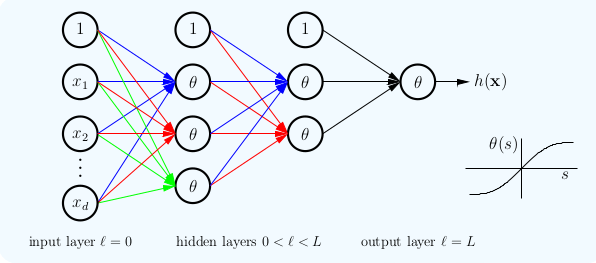
\includegraphics[scale=0.6]{img/grafo RRNN.png}
        \caption{Red Neuronal representada mediante un grafo. Imagen obtenida de \cite{data}. Notamos que el nodo del sesgo no le llega ninguna entrada}
        \label{fig:grafo rrnn prealimentada}
    \end{figure}
    
    La redes neuronales están organizadas en capas donde en cada una de ellas está comprendida por un conjunto de neuronas. El conjunto de neuronas $V$ se puede descomponer como unión disjunta de subconjuntos de neuronas, $V = \uplus V_{\ell=0}^L$ tal que cada subconjunto corresponde a los nodos de una única capa oculta. La arista en $E$ conecta algún nodo de $V_{\ell-1}$ con otro nodo de $V_{\ell}$ para algún $\ell \in [L]$. La capa $\ell = 0$ será llamada capa de entrada y contendrá $n+1$ neuronas donde $n$ es la dimensión del vector de entrada y la neurona restante será llamada sesgo y siempre contendrá el valor $1$. La última capa, $\ell = L$, es la capa de salida y determina el valor de la función. Finalmente las capas del medio serán llamadas capas ocultas. Usaremos el superíndice $\ell$ para referirnos a la capa, cada capa tiene dimensión $d^{(l)}$ que son el número de nodos presentes en la capa $\ell$. En la imagen \ref{fig:grafo rrnn prealimentada} podemos ver una representación gráfica de una pequeña red neuronal de cuatro capas. \\
    
   
    \begin{figure}[H]
        \centering
        \includegraphics[scale=0.8]{img/nodo nn.png}
        \caption{Interconexión entre dos nodos de dos capas contiguas. Fuente \cite{data}}
        \label{fig:nodo nn}
    \end{figure}
    
    
     Hagamos un poco de zoom sobre la topología de dos neuronas conectadas (Fig. \ref{fig:nodo nn}). En ella podemos ver dos nodos, representados por $i$ y $j$ en las capas $\ell -1$ y $\ell$ respectivamente. El nodo $v^{\ell}_j$ recibe una entrada, $s^{\ell}_j$, y emite una salida, $x^{\ell}_j$. La entrada $s^{\ell}_j$ consta de la salida del nodo $v^{\ell -1}_i$ de la capa anterior, $x^{\ell-1}_i$, multiplicado por los pesos asociados al enlace de ambos nodos, $w^{\ell}_{i,j}$.
    
    \begin{figure}[H]
        \centering
        \includegraphics[scale=0.8]{img/nodos nn.png}
        \caption{Interconexión entre capas ocultas. Fuente \cite{data}}
        \label{fig:nodos nn}
    \end{figure}
    
    
    La imagen \ref{fig:nodo nn} hace referencia a dos nodos conectados, pero en las redes neuronales son totalmente conectadas, es decir, todos los nodos de una capa se conectan con todos los nodos de la siguiente, por lo que la imagen \ref{fig:nodo nn} evoluciona a la imagen \ref{fig:nodos nn}. De esta manera, tenemos que la entrada a la capa $\ell$, $s^{\ell}$,  tiene dimensión $d^{\ell}$. La salida de esa misma capa, $x^{\ell}$, tiene dimensión $d^{\ell} + 1$. Los pesos de cada enlace los agrupamos en una matriz, $W^{\ell}$, con dimensión $(d^{\ell -1} + 1)\times d^{\ell}$. \\
    
    Una hipótesis $h \in \Hc_{NN}$ depende primordialmente de los pesos entre los enlaces, por lo que usualmente se denota como $h(x;w) = X^L$ donde $x = \{W^1,...,W^L\}$, enfatizando así la importancia de estos. \\
    
    Formalicemos la definiciones de conjunto de hipótesis de las redes neuronales, $\Hc_{NN}$ y redes neuronales prealimentadas. \\
    
    \begin{definicion}[Conjunto de hipótesis]
    Sea $L \in \N$, $d =(d^0,...,d^L) \in \N^L$, $W=(W^1,...,W^L)$ con $W^{\ell} \in \R^{(d^{\ell} + 1)\times d^{\ell}}$. El espacio de hipótesis de las redes neuronales prealimentadas viene dado por,
    \begin{equation}
        \Hc_{NN} = \{ h(x,W) : (L,d,W,\{\theta_t\}) \; implementa  \; h(x,W) = x^{(L)} \}
    \end{equation}
    \end{definicion}

    \begin{definicion}[Red Neuronal Prealimentada]
    Sea $L \in \N$, $d =(d^0,...,d^L) \in \N^L$, $W=(W^1,...,W^L)$ con $W^{\ell} \in \R^{(d^{\ell} + 1)\times d^{\ell}}$. Sean el conjunto de funciones $\{\theta^{\ell}: \ell \in \{1,...,L\}\}$ con $\theta$ una función de clase uno con valores de $\R^{d^{\ell-1}}$ en $\R^{d^{\ell}}$. Se define una red neuronal prealimentada como la cuaterna $[L,d,W,\{\theta^{\ell}\}]$ que implementa la función $h(x,W) = x^L$ a través de una conjunto finito de pasos de cálculo partiendo de unas condiciones iniciales,
    
    \begin{equation}
        \left\{ 
        \begin{array}{cc}
             
             
             x^0 = x & x \in \R^{d_0} \\
             
             x^{\ell} = \theta^{\ell}(s^{\ell}) & \ell \in \{1,...,L\} 
        
        \end{array}
        \right.
    \end{equation}
    
%    \begin{equation}
%        \left\{ 
%        \begin{array}{cc}
%             x^0 = 
%                \begin{bmatrix}
%                    1 \\ \theta^{\ell} (s^{\ell})
%                \end{bmatrix} 
%                & x \in \R^{d_0} \\
%             
%             x^{\ell} = 
%                 \begin{bmatrix}
%                    1 \\ \theta^{\ell}(s^{\ell}) 
%                 \end{bmatrix}
%             & \ell \in \{1,...,L\} 
%        \end{array}
%        \right.
%    \end{equation}
    
    \noindent donde
    \begin{equation}
        s^{\ell} = W^{\ell} x^{\ell - 1} + b^{\ell} \quad \ell \in \{1,...,L\}
    \end{equation}
    \end{definicion}


\section{Entrenamiento de Redes Neuronales}

    Cuando usamos una red neuronal que acepte una entrada $x_0$ y produzca una salida $x^L$, la información fluye hacia adelante a través de la red. La entrada $x_0$ proporciona la información inicial que luego se propaga a la unidades ocultas de cada capa para producir $x^L$. A esto se le llama \textit{forward propagation} o propagación hacia adelante. \\
    
    Durante el entrenamiento, este proceso tendrá una función de coste asociada $J$ que dependerá esencialmente de los pesos. El objetivo es calcular los pesos óptimos que minimizan dicha función. El algoritmo back-propagation permite que la información de la función de coste viaje hacia atrás a través de la red para calcular el gradiente. Este método surge de la necesidad de calcular de manera eficiente el gradiente ya que su principal inconveniente es su complejidad computacional. \\
    
    El back-propagation será usado en el algoritmo gradiente descendente, el cual se encarga de optimizar el valor de los pesos para minimizar así la función de coste. Este algoritmo requiere el cálculo del gradiente en cada iteración para movernos en dirección contraria. \\
    
    
    Antes de adentrarnos en faena con el entrenamiento de la red neuronal, comentemos algunas otras consideraciones importantes a tener en cuenta del entrenamiento. 
    \begin{itemize}
        \item \textit{Inicialización de los pesos}: Nunca se inicializan los pesos con valor cero o al mismo valor ya que de esa manera no habrá movimiento hacia el óptimo local en el gradiente descendente. Tampoco se deberán inicializar con valores muy grandes porque saturarían a la función sigmoidal y el gradiente se iría a cero. Lo correcto es una inicialización a pequeños valores aleatorios dados por una distribución gaussiana, $\mathcal{N}(0,\sigma_{\e}^2)$, de media cero y varianza $\sigma_{\e}^2$ cumpliendo $\sigma_{\e}^2 \underset{x_i}{max} || x_i||^2 << 1$. Para clasificación suele ser buena idea inicializar los pesos al valor obtenido después de aplicar un modelo de regresión. \\
        \item \textit{Criterio de parada}: Este criterio es de vital importancia para no aumentar de manera excesiva la complejidad en tiempo del entrenamiento. Hay muchos criterios tales como un número máximo de iteraciones, tamaño del gradiente, valor alcanzado en el error. Lo recomendable es usar una combinación de estos criterios.
    \end{itemize}
    
    
\subsection{Calculo del gradiente: Back-Propagation}

  El término back-propagation se suele malentender erróneamente como todo el algoritmo de aprendizaje de las redes neuronales. El back-propagation es un método para calcular el gradiente de manera eficiente para su posterior aplicación en el método del gradiente descendente o similares. Otro malentendido sobre el back-propagation es que solo se usa para calcular el gradiente de las redes neuronales, y esto tampoco es así. Es un método general, que además de emplearse en las redes neuronales se puede emplear en otros ámbitos ya que calcula las derivadas de cualquier función. En particular, calcula el gradiente $\nabla_{x}f(x,y)$ de una función arbitraria $f$, donde $x$ es un conjunto de variables las cuales queremos derivar, e $y$ es un conjunto de variables de las cuales depende la función pero no queremos derivar. En machine learning, el gradiente que se suele calcular es el de la función de coste, pero este algoritmo no tiene por qué usarse particularmente ahí. Si otras tareas de ML requieren calcular las derivadas de otras funciones, también puede emplearse esta técnica. El back-propagation puede generalizarse para salidas múltiples, pero para una mayor simplicidad, vamos a considerar que $f$ solo tiene una salida. \\ 
        

    Este algoritmo consiste en aplicar la regla de la cadena en cada nodo del grafo computacional para calcular el gradiente de manera eficiente. Se logra la eficiencia gracias a que no se repiten cálculos ya realizados y a una reordenación de los mismos. \\
        
    Para entenderlo mejor, vamos a dar un pequeño ejemplo de como se haría para el caso de un grafo computacional sencillo y después lo extenderemos al caso de redes neuronales. Considerar un grafo computacional cuya salida es un único escalar denotado como $u$. Queremos calcular el gradiente con respecto a los $n$ nodos del grafo denotados como $u^{(i)}$ con $i \in \{1,2,...,n\}$.  En otras palabras, queremos calcular $\frac{\partial u}{\partial u^{(i)}}$ para todo $i \in \{1,...,n\}$. Como ejemplo, vamos a considerar el grafo computacional de la figura \ref{fig:bp_grafo} donde cada nodo es una variable de entrada y se tiene $w, \; u^{(2)} = x = f(w), \; u^{(3)} = y = f(x)$ y $z = f(y)$ siendo esta última la variable de salida. \\
        
        \begin{figure}[htpb]
            \centering
            \includegraphics[scale=0.5]{img/backpropagation1.png}
            \caption{Grafo computacional que resulta del cálculo de la función f(f(f(w))) siendo $w \in \mathbb{R}$ y $f:\mathbb{R} \rightarrow \mathbb{R}$ una función real de variable real. Esta figura muestra el problema de la repetición de operaciones cuando se calcula el gradiente.}
            \label{fig:bp_grafo}
        \end{figure}
        
        \begin{figure}[htpb]
            \centering
            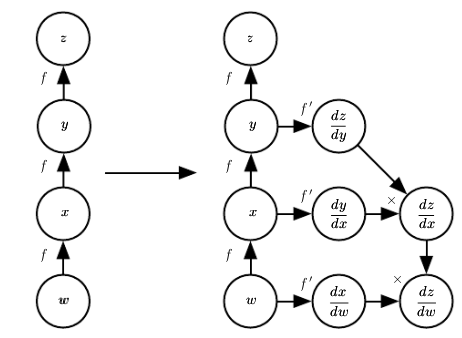
\includegraphics[scale=0.5]{img/grafo2.png}
            \caption{(Izquierda) Grafo que representa la función compuesta $z = f(f(f(w))). (Derecha)$ Grafo tras aplicar el algoritmo de \textit{back-propagation}. Este grafo representa el resultado deseado.}
            \label{fig:bp_grafo2}
        \end{figure}
        
    Para calcular $\frac{\partial z}{\partial w}$ aplicamos la regla de la cadena obteniendo
        
        \begin{equation}
            \begin{aligned}
                    \frac{\partial z}{\partial w} & = \frac{\partial z }{\partial y}\frac{\partial y}{\partial x}\frac{\partial x}{\partial w}\\
                    & = f'(y) f'(x) f'(w) \\
                    & = f'(f(f(w))) f'(f(w)) f'(w)
            \end{aligned}
        \end{equation}
        
    \noindent donde se observa que se realizan algunos cálculos repetidos, en este caso, se evalúa dos veces la función $f$ en la variable $w$. Si el grafo fuera mucho más complejo, tendríamos muchos más de estos cálculos repetidos provocando una disminución del tiempo considerable a la hora de computarlo. Se podría mejorar la eficiencia en tiempo si en memoria se guardarse el valor de estos cálculos y se usasen para operaciones futuras. \\
        
    Vamos a suponer que los nodos del grafo están ordenados y en cuyo caso podremos calcular la salida una detrás de otra. Cada nodo $u^{(i)}$ está asociado a una operación $f^{(i)}$ y se calcula evaluando la función 
        
        \begin{equation}
            u^{(i)} = f(\mathbb{A}^{(i)}) 
        \end{equation}

    \noindent donde $\mathbb{A}^{(i)}$ es el conjunto de todos los nodos padres que intervienen en el cálculo de la expresión $u^{(i)}$. También llamaremos por $Pa(u^{(i)}) = \{ j \; : b^{(j)} \in \mathbb{A}^{(i)}\}$ al conjunto de los índices de los nodos padre de $u^{(i)}$. Para el cálculo de las distintas derivadas usaremos la regla de la cadena
        
        \begin{equation}
            \frac{\partial u}{\partial u^{(j)}} = \sum_{i/j \in Pa(u^{(i)})} \frac{\partial u}{\partial u^{(i)}} \frac{\partial u^{(i)}}{\partial u^{(j)}}
        \end{equation}
        
    Llamamos $\mathcal{G}$ al grafo de cómputo de la función $f$, en nuestro ejemplo sería el grafo de la figura \ref{fig:bp_grafo}. Para realizar \textit{back-propagation} podemos construir un grafo computacional que depende de $\mathcal{G}$ y en donde añadimos nodos extra. Denotamos a dicho grafo como $\mathcal{B}$, los cálculos en $\mathcal{B}$ se realizan con el orden inverso que tienen en $\mathcal{G}$ y cada nodo de $\mathcal{B}$ calcula la derivada $\frac{\partial u}{\partial u^{(i)}}$ asociada al grafo hacia adelante del nodo $u^{(i)}$. El grafo $\mathcal{B}$ contiene exactamente una arista por cada arista que tenga $\mathcal{G}$ desde el nodo $u^{(j)}$ al nodo $u^{(i)}$, de este modo, si desde el nodo $u^{(j)}$ al nodo $u^{(i)}$ hay 5 aristas, entonces el nuevo grafo contendrá $5$ nodos extra enlazados con sus respectivas aristas, cada nodo representa una derivada. La arista de $u^{(j)}$ a $u^{(i)}$ está asociada al cálculo de $\frac{\partial u^{(i)}}{\partial u^{(j)}}$. Además, se realiza un producto para cada nodo entre el gradiente calculado y respecto a los nodos $u^{(i)}$ que son los hijos del nodo $u^{(j)}$. En nuestro ejemplo, el cálculo del grafo $\mathcal{B}$ quedaría como el de la imagen (derecha) de \ref{fig:bp_grafo2}. A continuación vamos a mostrar un algoritmo de una versión simplificada del \textit{backpropagation} que calcula las derivadas de $u^{(n)}$ con respecto a las variables en el grafo. \\
    
    En el contexto de redes neuronales, se calcula el gradiente con respecto los pesos $W$ y los sesgo $b$ de la función de coste $J(w,b) = \frac{1}{N} \sum_{i=1}^N \ell(h_{w,b},y_i) + \lambda \Omega(w,b)$ con $w = [W_1,...,W_L]$ donde el segundo sumando indica el término de regularización. Para una mayor simplicidad vamos a incluir los sesgos en el vector $W$ tomando como índice el cero, por lo que el vector $x$ en este caso tendrá una componentes más con valor constantemente igual a $1$. \\
	  
	
    \subsubsection{Propagación hacia adelante (Feed Forward)}
        
        Esta es la primera parte del algoritmo, cuya finalidad principal es calcular el grafo $\mathcal{G}$ \eqref{eq:grafo feed forward} que en términos de redes neuronales se traduce en calcular la función que implementa la red neuronal. \\
        
        \begin{equation} \label{eq:grafo feed forward}
            x^0 \overset{W^1}{\longrightarrow} s^1 \overset{\theta^1}{\longrightarrow} x^1 \overset{W^2}{\longrightarrow} s^2 \overset{\theta^2}{\longrightarrow} x^2 \cdots x^{L-1} \overset{W^L}{\longrightarrow} s^L \overset{\theta^L}{\longrightarrow}x^L
        \end{equation}
        
        	\begin{algorithm}[H]
        	\label{alg:forward}
	        \caption{Propagación hacia adelante para calcular la función de coste a través de una red neuronal profunda típica}
	        \KwData{$L$: Network Deep}
	        \KwData{$x$: input}
	        \KwData{$y$: target}
	        \KwData{y: target}
	        \KwData{$\{\theta^i\}: i \in \{1,...,L\}$}
	        \KwData{$W^i$: $i \in \{0,1,...,L\}$ matrices de pesos (con sesgos)}
	        \KwResult{$(x_i)_{1,...,L},(s_i)_{1,...,L}$}
	        
	        $x^0 \leftarrow x$ \; 
	        \ForEach{$k \in \{1,...,L\}$}{
	            $s^k \leftarrow  W^k x^{k-1}$\;
	            $x^k \leftarrow \begin{bmatrix}
                    1 \\ \theta^{\ell} (s^{\ell})
                \end{bmatrix} $\;
	            }
	       $h(x,W) \leftarrow x^L$\;
	       $J = L(h(x,W),y) + \lambda \Omega(W)$
	       \end{algorithm}
	       
	                       
	       
	       
	       \begin{figure}[H]
	           \centering
	           \includegraphics[scale=0.7]{img/propagacion forward.png}
	           \caption{Representación de la propagación hacia adelante en una red neuronal prealimentada}
	           \label{fig:esquema forward}
	       \end{figure}
        
        
    \subsubsection{Propagación hacia atrás (Back-Propagation)}
        
        
        Antes de entrar de lleno con el algoritmo, especifiquemos la notación. Definimos la \textit{sensibilidad} como
        
        \begin{equation}\label{eq:sensibity}
            \delta^{\ell} = \frac{\partial L}{\partial s^{\ell}}
        \end{equation}
        
        \noindent La sensibilidad cuantifica cómo cambia $L$ con respecto a $s^{\ell}$. Usando la sensibilidad podemos escribir la derivada parcial con respecto la matriz de pesos $W^{\ell}$ como,
        
        \begin{equation}\label{eq:partial L partial W}
            \frac{\partial L}{\partial W^{\ell}} = \frac{\partial L}{\partial s^{\ell}} \frac{\partial s^{\ell}}{\partial W^{\ell}} = x^{\ell - 1}(\delta^{\ell})^T
        \end{equation}
        
        

        
        
        \noindent La derivada parcial del término de la izquierda es una matriz de dimensión ${(d^{\ell -1} + 1)\times d^{\ell}}$ y no es difícil probar que dicha matriz se obtiene con el producto de los dos vectores del término de la derecha. La imagen \ref{fig:backpro esquema} muestra que en la salida de la capa $\ell + 1$ el vector $\delta^{\ell + 1}$ el cual es multiplicado por la matriz de pesos $W^{\ell + 1}$ se suma y se le pasa como entrada a las neuronas de la capa $\ell$. Estos nodos multiplican dicha entrada por el jacobiano $(J_{\theta^{\ell}})_{s^{\ell}}$ para obtener $\delta^{\ell}$. Denotando $\odot$ la multiplicación elemento a elemento de dos vectores tenemos que,
        
        \begin{equation}
            \delta^{\ell} = (J_{\theta^{\ell}})_{s^{\ell}} \odot [W^{\ell + 1} \delta^{\ell + 1}]_1^{d^{\ell}}
        \end{equation}
        
        \noindent donde el vector $[W^{\ell + 1} \delta^{\ell + 1}]_1^{d^{\ell}}$ representa las componentes $1,...,d^{\ell}$ del vector $W^{\ell + 1} \delta^{\ell + 1}$ excluyendo la componente del sesgo la cual tiene índice cero. Esta fórmula no es nada extraña ni la hemos sacado de la manga. La sensibilidad del error en la capa $\ell$ es proporcional a la pendiente de la función de activación de la capa $\ell$ (mayor pendiente significa que un pequeño cambio en $s^{\ell}$ tendrá un mayor impacto en $s^{\ell + 1}$), al tamaño de los pesos que salen de la capa (mayores pesos significan que un menor cambio en $s^{\ell}$ tendrá más impacto en $s^{\ell + 1}$) y a la sensibilidad de la capa siguiente ( un cambio en la capa $\ell$ afecta a la entrada de la capa $\ell + 1$ así que si el error es mas sensible a la capa $\ell + 1$ entonces tendrá aún más sensible a la capa $\ell$). \\
        
   
        La salida de capa capa $x^{\ell}$ se calcula en la propagación hacia adelante usando la salida de la capa anterior $x^{\ell - 1}$. Para calcular la sensibilidades basta con recorrer el grafo de la red neuronal hacia atrás ya que para calcular $\delta^{\ell}$ necesitamos $\delta^{\ell + 1}$. Esta idea se muestra en la figura \ref{fig:backpro esquema}, quedando el grafo computacional de la siguiente manera
        
        \begin{equation}
            \delta^{1} \leftarrow \delta^{2} \cdots \leftarrow \delta^L
        \end{equation}
   
        \begin{figure}[htpb]
            \centering
            \includegraphics[scale=0.7]{img/backpro esquema.png}
            \caption{Representación esquemática de la propagación hacia atrás}
            \label{fig:backpro esquema}
        \end{figure}
        
        El algoritmo queda como sigue,
        
        \begin{algorithm}[H]
	       \label{alg:feedforward}
	        \caption{Propagación hacia atrás}
	        \KwData{$[L,d,W,b,\{\theta^i\}]$ red neuronal prealimentada}
	        \KwData{$x$: input}
	        \KwData{$y$: target}
	        \KwData{y: target}
	        \KwResult{$\nabla_W L$}
	        
	        $(s^i)_{1,...,L},(x^i)_{0,...,L} \leftarrow ForwardPropatagion$ \;
	        $\delta^L \leftarrow \frac{\partial L}{\partial s^L}$ \; 
	        \ForEach{$\ell$ $\in$ $\{L-1,...,1\}$}{
	            $\delta^{\ell} = (J_{\theta^{\ell}})_{s^{\ell}} \odot [W^{\ell + 1} \delta^{\ell + 1}]_1^{d^{\ell}}$\;
	            $\frac{ \partial L}{\partial W^{\ell}} = x^{\ell - 1} (\delta^{\ell})^T$
	            }
	   \end{algorithm}
        

    \subsection{Optimización a través del Gradiente descendente}

    Fijada una función de coste y un algoritmo eficiente para el cálculo del gradiente introducimos el método de optimización que se aplica en las redes neuronales, el gradiente descendente. Este método fue propuesto inicialmente en $1847$ por Cauchy \cite{cauchy1847methode}, y no fue hasta casi 100 años después que se demostró su convergencia gracias a Haskell Curry \cite{curry1944method}. \\
    
    La intuición geométrica que subyace detrás de esta técnica es la siguiente. Veamos la función que queremos minimizar como una superficie en el espacio. En un instante de tiempo cero, partimos de la posición $w(0)$ de la superficie, y en cada instante de tiempo nos vamos moviendo sobre ella. El objetivo es descender de la superficie hasta llegar un punto en el que nos movamos en la dirección en la que nos movamos, no consigamos descender más. También podemos considerar el movimiento de descenso como aquel que haría una pelota si la colocásemos en una superficie $2$-dimensional gracias a la gravedad, ésta descendería hasta llegar a un punto de equilibro, entendido como un mínimo local. \\
    
    Vamos a considerar un campo escalar $f:S \subset \R^n \to \R$ continuo y derivable en su dominio con derivada continua en el interior de $S$. Su función gradiente $\nabla f$ es un campo vectorial y apunta en la dirección en que la derivada direccional es máxima por lo que la dirección en la que la función desciendo más rápido viene dada por,
    
    \begin{equation}
        -\eta \nabla f(w_1,...,w_n) = -\eta \Big( \frac{\partial f}{\partial w_1} (w_1,...,w_n),...,\frac{\partial f}{\partial w_n}(w_1,...,w_n) \Big)
    \end{equation}

    \noindent donde $\eta$ es un factor de proporcionalidad más conocido en el mundo del aprendizaje automático como tasa de aprendizaje. De este modo el algoritmo consiste en partir de unas condiciones iniciales $w_0$ y de manera iterativa calcular el vector opuesto del gradiente y avanzar en esa dirección una distancia marcada por la tasa de aprendizaje. Las ecuaciones quedan como siguen,
    
    \begin{equation}
        w_i = x_{i-1} - \eta \nabla f(w_{i-1}) \qquad w_i \in \R^n 
    \end{equation}


    Hay que tener siempre en mente que cuando aplicamos esta técnica, obtendremos un mínimo local que por lo general no será global. \\
    
    \subsubsection{Variantes del gradiente descendente}
    
    En el panorama del aprendizaje automático, tendremos un conjunto de entrenamiento conformado por varios elementos (vectores) por lo que calcularemos la media aritmética de los gradientes de la función de pérdida para cada uno de esos elementos. Para ello, evaluaremos la función de coste para cada ejemplo de entrenamiento antes de actualizar el gradiente, lo que computacionalmente en tiempo es una barbaridad. Como contramedida, solo se emplea un solo ejemplo de entrenamiento en cada actualización, esta variación del gradiente descendente recibe el nombre de \textit{gradiente descendente estocástico}. \\
    
    
        \begin{algorithm}[H]
	       \label{alg:SGD}
	        \caption{Gradiente Descendente Estocástico (SGD)}
	        \KwData{$W_0$ condiciones iniciales}
	        \KwData{$\eta$: tasa de aprendizaje}
	        \KwData{$S$: conjunto de entrenamiento}
	        \KwData{$L$: función de perdida}
	        \KwData{$n\_epochs$: numero de epocas}
	        \KwResult{$w$ pesos finales}
	        

    	       \ForEach{$(x,y)$ $\in$ $S$}{
    	           $w \leftarrow w - \eta \nabla L(h(x,w),y)$
    	           }
	           
	   \end{algorithm}
	   
	   
	 Esta variación del gradiente descendente nos sitúa en el extremo opuesto que la versión en donde se evalúan todos los ejemplos de entrenamiento y aplicamos la media. Por lo que esta aproximación no va a ser tan fidedigna como la otra, así que, como alternativa surgió el \textit{descenso del gradiente estocástico con minilotes}. Consideramos una partición disjunta del conjunto de entrenamiento y a cada subconjunto lo llamamos minilote. Entonces este método consiste en actualizar los pesos una vez se haya evaluado todos los ejemplos de dicho minilote. Así según el tamaño del minilote, buscamos un compromiso entre la robustez del gradiente descendente y la eficiencia del SGD. \\
	 
	 Algo a tener en cuenta y a lo cual le hemos restado importancia hasta ahora es la tasa de aprendizaje $\eta$. Su correcto valor es un factor clave, en la en la imagen $\ref{fig:lr}$ podemos ver distintos escenarios según su valor. Una tasa de aprendizaje pequeña consigue que el gradiente descendente avance poco a poco necesitando muchas iteraciones para la convergencia. Una tasa de aprendizaje grande, puede ocasionar que la convergencia sea inestable o incluso saltarnos el óptimo. Otro escenario es que la tasa de aprendizaje sea una función que vaya variando, de tal modo que al principio tenga valores grandes para acelerar la convergencia y conforme avanzamos en iteraciones tome valores pequeños para no escaparnos del óptimo. \\
	 
	 Este última método motiva una amplia gama de variaciones en el gradiente descendente que se centran en cómo modificar la tasa de aprendizaje. De este modo surgen variantes como AdaGrad, Adam, RMSProp...
	 
	 \begin{figure}[H]
	     \centering
	     \includegraphics[scale=0.5]{img/learningrate.png}
	     \caption{Escenarios que presenta la elección de la tasa de aprendizaje}
	     \label{fig:lr}
	 \end{figure}


       
        
        
\section{Función de Activación}
    
    Las funciones de activación son transformaciones que por lo general son no lineales que se aplican al producto escalar de los pesos por las características en cada neurona para dar la salida. La no linealidad aporta una mayor variedad y mejores aproximaciones. Veamos las más comunes usadas en la práctica. \\
    
    \begin{center}
        \textbf{Función sigmoidal} \\
    \end{center}
    
        Esta función es de la forma
        
        \begin{equation}
            \sigma(x) = \frac{1}{1 + e^{-x}}
        \end{equation}
        
        \noindent y claramente es no lineal. Tiene por dominio la recta real, pues el denominador no se anula en ningún punto, haciéndola una función continua, además es diferenciable. Toma valores en el intervalo $[0,1]$ y presenta dos asíntotas horizontales en el infinito,
        
        \begin{equation}
            \sigma(x) \overset{x \to -\infty}{\longrightarrow}  0 \qquad  \sigma(x)\overset{x \to \infty}{\longrightarrow}  1
        \end{equation}
        
        Esta función es muy útil pues la podemos emplear para transformar un escalar en una probabilidad colapsando a cero o a uno según la magnitud de éste, por este motivo se suele emplear en la capa de salida (aunque también es común usarla en las neuronas de las capas ocultas). La gráfica la presentamos en la figura \ref{fig:grafica sigmoidal}. \\
        
        Un inconveniente es que estas funcionan saturan y destruye los gradiente durante el proceso de entrenamiento. Esto es debido a que cuando la neurona satura el producto escalar en algunas de las colas, ya sea $0$ ó $1$ el gradiente en esas regiones es prácticamente nulo. Durante el proceso de retropropagación, puede resultar bastante peligroso por lo que se podría desvanecer. \\
        
        Por otro lado y relacionado con el motivo anterior, hay que ser muy cuidadosos con la inicialización de los pesos de las neuronas que usen este tipo de función de activación para evitar dicha saturación en las colas. Ya que si los pesos son muy grandes en términos absolutos, la red no va a aprender debido al desvanecimiento del gradiente. \footnote{El problema del desvanecimiento del gradiente lo comentaremos en el capítulo de Redes Neuronales Recurrentes, para más información ir a la sección \ref{seccion:sorpresa}} \\
        
        Otro problema es que la salida no está centrada en el cero, esto puede originar un comportamiento indeseado en las actualizaciones del gradiente de los pesos. \\
        
        \begin{figure}[H]
            \centering
            \includegraphics[scale=0.5]{img/sigmoide.png}
            \caption{Gráfica función sigmoidal. \href{https://ml4a.github.io/images/figures/sigmoid.png}{Fuente}}
            \label{fig:grafica sigmoidal}
        \end{figure}
        
        
        
        
        
    \begin{center}
        \textbf{Función tangente hiperbólica} \\
    \end{center}
    
        La gráfica de la función la presentamos en \ref{fig:grafica tanh}. Es otra función no lineal cuya expresión viene dada por 
        
        \begin{equation}
            \tanh(x) = \frac{e^x - e^{-x}}{e^x + e^{-x}}
        \end{equation}
        
        \noindent también la podemos poner en términos de la función sigmoidal,
        
        \begin{equation}
            \tanh(x) = 2 \sigma(2x) - 1
        \end{equation}
        
        Al igual que la función sigmoidal, tiene de dominio toda la recta real, pero ahora los valores que toma están comprendidos en el intervalo $[-1,1]$ presentando una asíntota vertical en el infinito hacia esas colas, esto es,
        \begin{equation}
            \tanh(x) \overset{x \to -\infty}{\longrightarrow}  -1 \qquad  \tanh(x)\overset{x \to \infty}{\longrightarrow}  1
        \end{equation}
        
        \noindent Esta vez, tenemos que la función está centrada en el cero, por lo que aunque la salida de esta función se sature no tendremos el problema que comentamos con la función sigmoidal sobre el comportamiento indeseado en la actualización del gradiente de los pesos. Por este motivo se prefiere la no linealidad de esta función frente a la sigmoidal, aunque sea un simple escalado de la anterior. \\
    
        \begin{figure}[H]
            \centering
            \includegraphics[scale=0.3]{img/tanh.png}
            \caption{Gráfica función tangente hiperbólica \href{https://production-media.paperswithcode.com/methods/Screen_Shot_2020-05-27_at_4.23.22_PM_dcuMBJl.png}{Fuente}}
            \label{fig:grafica tanh}
        \end{figure}
        
        
    \begin{center}
        \textbf{Función ReLu} \\
    \end{center}
    
        La unidad lineal rectificada se ha hecho muy popular en los últimos años. Su expresión viene dada por
        \begin{equation}
            f(x) = max(0,x)
        \end{equation}
        
        \noindent Esta función se puede ver como un simple umbral en cero. Su gráfica viene dada por la imagen \ref{fig:grafica relu}. El uso de esta función de activación presenta varias ventajas así como desventajas.
        
        \begin{itemize}
            \item Ventajas:
            \begin{enumerate}
                \item Acelera en gran medida la convergencia del escenso del gradiente estocástico en comparación con las funciones tanh y sigmoidal debido a su forma no lineal y a no saturar los valores.
                \item En comparación con otras funciones de activación que implican operaciones costosas como exponenciales, esta función se puede implementar de manera muy simple y con poco coste.
            \end{enumerate}
            \item Desventajas: Estas funciones pueden ser frágiles durante el entrenamiento y pueden desvanecerse. Por ejemplo, imaginemos un gradiente que discurra por una neurona con esta función de activación, podría darse el caso en el que los pesos se actualicen de manera que la neurona no vuelva a activarse en ningún punto. Si esto pasara, entonces el gradiente que pasa por esta neurona será siempre nulo a partir de ese punto. Se ha llegado a observar en algunos casos que hasta el $40\%$ de la red puede desvanecerse, esto es, neuronas que nunca se activan en todo el conjunto de datos de entrenamiento en el caso de que la tasa de aprendizaje sea algo elevada. Para un ajuste adecuado de la tasa de aprendizaje, esto no debiera de ocurrir con tanta facilidad.
            
        \end{itemize}
    
    
        \begin{figure}[H]
            \centering
            \includegraphics[scale=0.55]{img/relu.png}
            \caption{Gráfica función ReLu \href{https://miro.medium.com/max/357/1*oePAhrm74RNnNEolprmTaQ.png}{Fuente}}
            \label{fig:grafica relu}
        \end{figure}
        
        
    \begin{center}
        \textbf{Función Leaky ReLu} \\
    \end{center}
    
        Esta función de activación cuya gráfica la podemos encontrar en la imagen \ref{fig:leakyrelu} es un intento de solucionar el problema de la ReLu comentado anteriormente. En lugar de que la función tome el valor cero, tomará una pequeña pendiente positiva. La expresión viene dad por
        \begin{equation}
            f(x) = max(\alpha x, x)
        \end{equation}
        \noindent donde $\alpha$ es una constante que suele tomar valores del orden de $10^{-3}$
        

        
        \begin{figure}[H]
            \centering
            \includegraphics[scale=0.55]{img/leakyrelu.png}
            \caption{Gráfica función Leaky ReLu \href{https://miro.medium.com/max/398/1*FDOyQlRurCK7mWU5i0Ly_w.png}{Fuente}}
            \label{fig:leakyrelu}
        \end{figure}
    
    \begin{center}
        \textbf{Otras Variante de ReLu: Elu y Selu} \\
    \end{center}
    
        La función Leaky ReLu no es la única alternativa que se propuso frente a ReLu, tenemos otras muchas variantes como Elu y Selu. Sus gráficas las podemo ver en la figura \ref{fig:grafica variante relu}. La función Elu viene dada por 
        \begin{equation}
            Elu(x) = max(\alpha(e^x -1),x)
        \end{equation}
        
        \noindent donde $\alpha > 0$ es una contante que al igual que el caso de la funcón Leaky Relu, toma valores pequeños. En cambio la función Selu viene dada por 
        
        \begin{equation}
            Selu(x) = max(\alpha \lambda(e^x - 1,x))
        \end{equation}
        
        \noindent donde $\lambda \approx 1.0507$ y $\alpha \approx 1.6732$. 

        
        
        \begin{figure}[H]
            \centering
            \includegraphics[scale=0.4]{img/Variante ReLu.png}
            \caption{Variantes ReLu \href{https://www.researchgate.net/profile/Alberto-Marchisio/publication/328878703/figure/fig2/AS:691988286423047@1541994272922/Behavior-of-ReLU-ELU-and-SELU-activation-functions.ppm}{Fuente}}
            \label{fig:grafica variante relu}
        \end{figure}
    
    
    
    \begin{center}
        \textbf{Función MaxOut} \\
    \end{center}
    
    Es otro tipo de función de activación que generaliza la ReLu y su versión Leaky ReLu. Su expresión viene dada por 
    \begin{equation}
        maxout = max(w^T_1x+b_1,w^T_2x+b_2)
    \end{equation}
    
    \noindent Por lo que esta función de activación goza de todas las ventajas que presenta la ReLu y no tiene sus inconvenientes. Pero presenta un nuevo problema al duplicar los parámetros para cada neurona. 
    



\endinput

